% Method descriptions of the implemented A/C experiments; requires amsmath,
% amssymb, graphicx and booktabs. Paths are relative to the repository root.
\section{No-Observation Operator Flow Matching}
Let $H$ denote the normalized building-height map, $T$ the transmitter-location
indicator, $B$ the target beam map, and $a=(n,f,\theta)$ the known array
configuration. The target $y$ is a normalized radio-power map on the model
grid. During training, $y$ and the validity mask $M$ provide supervision;
neither the target map nor a same-scene auxiliary radio map is an inference
input. We study two implementations, A and C, under the same flow-matching
backbone and target data protocol.

\subsection{Variant A: Beam-Conditioned Velocity with a Fixed Source}
\begin{figure}[t]
 \centering
 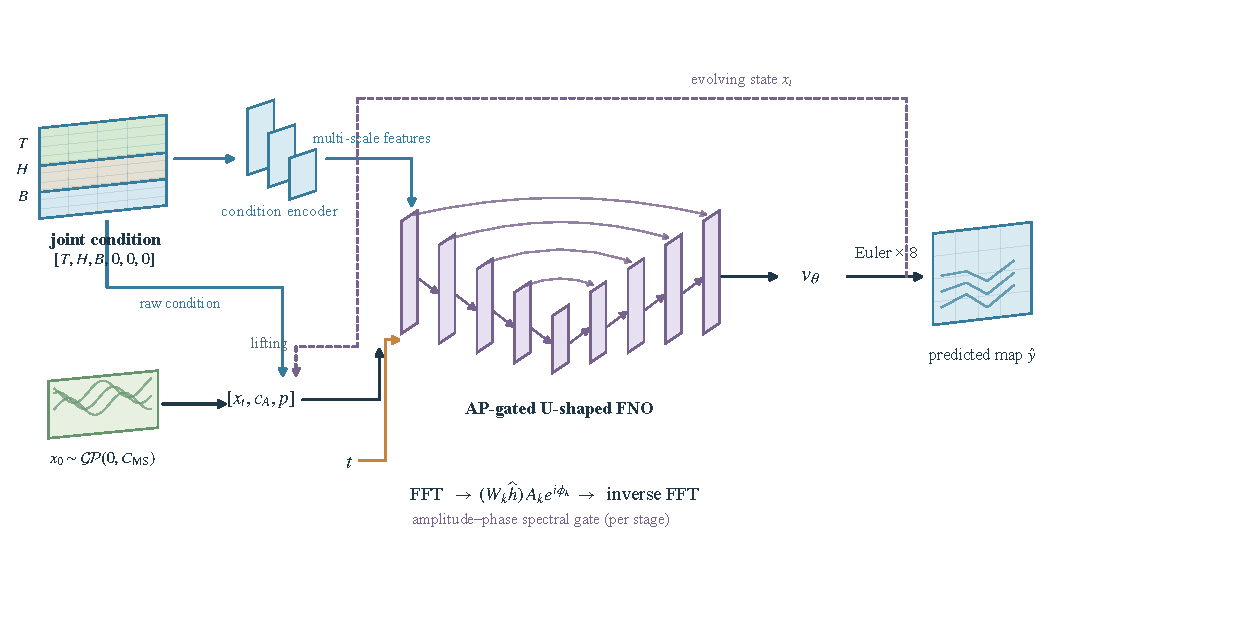
\includegraphics[width=\linewidth]{assets/method_a.pdf}
 \caption{Variant A: transmitter, height, and target beam maps form a joint
 condition for a Fourier velocity field that transports a multiscale source.
 Feature planes and fields are schematic.}
 \label{fig:ac-method-a}
\end{figure}
The A model uses the condition $c_A=[T,H,B,0,0,0]$. Its source is a
zero-mean multiscale Mat\'{e}rn random field, independent of the scene and
beam. For spatial separation $r$, the component covariance is
\begin{equation}
 C_{\ell}(r)=\begin{cases}
 (r/\ell)K_1(r/\ell), & r>0,\\ 1, & r=0,
 \end{cases}
 \quad C_{\rm MS}=\frac{1}{3}\sum_{\ell\in\{2,8,32\}} C_{\ell},
 \label{eq:ac-matern}
\end{equation}
where $K_1$ is the modified Bessel function of the second kind and length
scales are in model-grid pixels. The sampler uses a positive-semidefinite
checked circulant embedding. In the paired A/C implementation, independent
$z_{\rm MS}\sim\mathcal{GP}(0,C_{\rm MS})$ and
$z_{\ell}\sim\mathcal{GP}(0,C_{\ell})$ yield
\begin{equation}
 x_0^A=\sqrt{0.75}\,z_{\rm MS}+
 \frac{0.5}{\sqrt{3}}\sum_{\ell\in\{2,8,32\}}z_{\ell}.
 \label{eq:ac-a-source}
\end{equation}
Thus $x_0^A$ has covariance $C_{\rm MS}$. For $t\sim U[0,1]$,
\begin{equation}
 x_t=(1-t)x_0+t y,\qquad u_t=y-x_0,\qquad
 \widehat u_t=v_{\vartheta_A}(x_t,t,c_A).
 \label{eq:ac-flow}
\end{equation}
The velocity network is a U-shaped multiscale Fourier operator. A condition
encoder supplies multiresolution features; each operator stage combines
conditioned attention, a truncated spectral convolution, a local linear
branch, time embedding, and a residual connection. In an AP-gated stage,
for retained Fourier mode $k$, the learned gate and spectral update are
\begin{align}
 g_{\vartheta}(k)&=\left[1+0.5\tanh a_{\vartheta}(k)\right]
 \exp\!\left(i\tfrac{\pi}{4}\tanh b_{\vartheta}(k)\right),\\
 \widehat s_o(k)&=g_{\vartheta,o}(k)\sum_i W_{io}(k)\widehat h_i(k).
 \label{eq:ac-gate}
\end{align}
The gate networks receive normalized spectral features of the state and
condition, their relative phase features, mode coordinates, and the time
embedding. The gate is set to one on the implementation's excluded real-FFT
boundary columns. This is modulation of latent Fourier features, rather than
an estimate of the physical electromagnetic phase.

\subsection{Variant C: Structured Source and Beam-Conditioned Noise}
\begin{figure}[t]
 \centering
 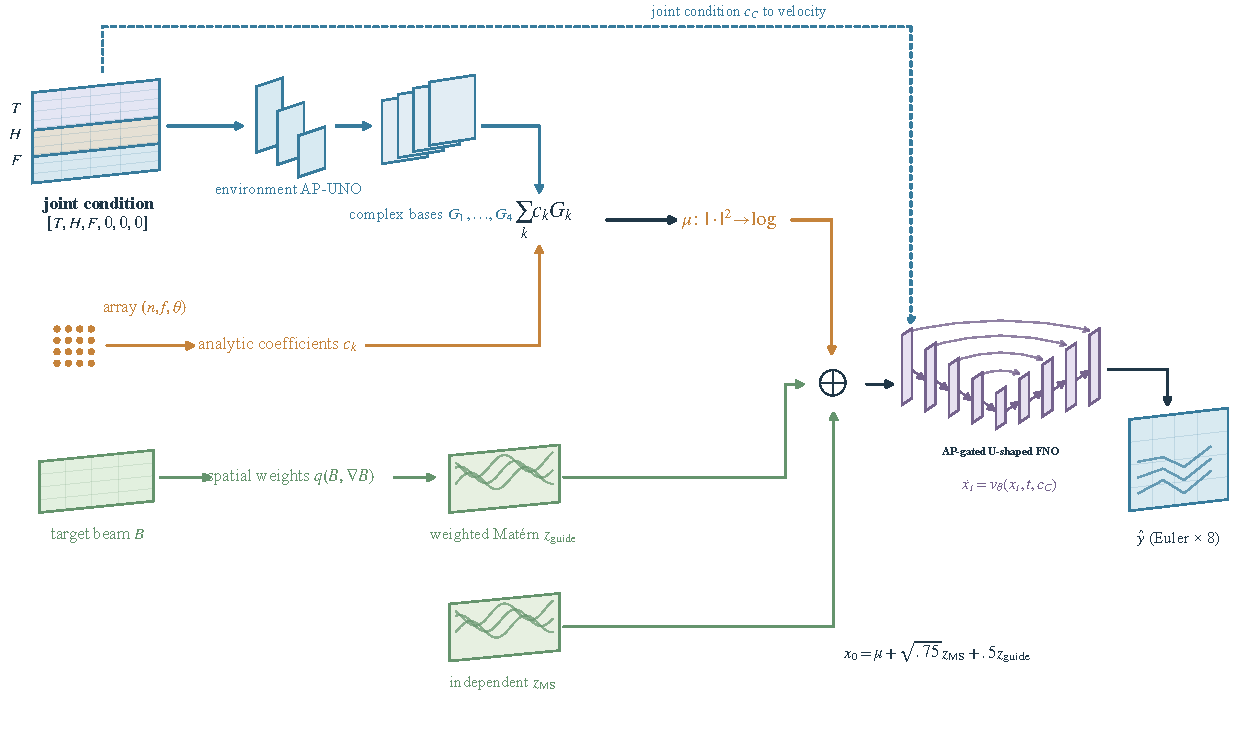
\includegraphics[width=\linewidth]{assets/method_c.pdf}
 \caption{Variant C: environmental features and analytic excitation form a
 source mean, while the beam map modulates the source covariance. Feature
 planes and fields are schematic.}
 \label{fig:ac-method-c}
\end{figure}
C separates the direct beam-map input from the velocity condition. It uses
$c_C=[T,H,F,0,0,0]$, where $F=\log(f/f_{\rm ref})$ is broadcast spatially
and $f_{\rm ref}=6.7$ GHz. An environmental AP-gated U-shaped Fourier network
maps $(T,H,F)$ to four complex latent basis maps
$G_k(H,T,F;p)$, $k=1,\ldots,4$. These bases are learned from power-map
supervision and are not identified as measured physical paths.

For an $n\times n$ array, let $r_m$ be the implemented half-wavelength
element offset and $w_m(n,\theta)$ the normalized steering weight. For the
four fixed basis directions $\varphi_k\in\{-30^\circ,-10^\circ,
10^\circ,30^\circ\}$, the analytic excitation coefficient is
\begin{align}
 d_k&=(\cos\varphi_k,\sin\varphi_k,0),\\
 c_k(a)&=\sum_{m=1}^{n^2}\overline{w_m(n,\theta)}\,
 \sqrt{10^{g_k/10}}\exp\!\left(i\frac{2\pi f}{c_0}r_m^{\mathsf T}d_k\right),\\
 g_k&=8-\min\!\left\{12(\varphi_k/65^\circ)^2,30\right\}.
 \label{eq:ac-excitation}
\end{align}
The structured field and source mean are computed as
\begin{equation}
 U(p)=\sum_{k=1}^{4}c_k(a)G_k(p),\qquad
 \mu(p)=\frac{10\log_{10}\!\left[(\lambda_f/4\pi)^2|U(p)|^2+10^{-30}\right]+300}{300},
 \label{eq:ac-mean}
\end{equation}
where $\lambda_f=c_0/f$ and the implementation scales each complex network
output by $1/100$ when forming $G_k$.

The normalized beam map $B$ also constructs a distribution over model-grid
positions. Let $N$ be the number of grid cells and $s_g$ the fixed training
set 95th percentile of positive beam-gradient magnitudes. With
$\alpha=\operatorname{softplus}(a_0)$ and
$\beta=\operatorname{softplus}(b_0)$, define
\begin{align}
 d(p)&=\operatorname{clip}\!\left(\frac{\lVert\nabla B(p)\rVert}{\max(s_g,10^{-6})},0,1\right),\\
 q(p)&=0.8\,\frac{\exp[\alpha B(p)+\beta d(p)]}
 {\sum_{u}\exp[\alpha B(u)+\beta d(u)]}+\frac{0.2}{N},\quad
 \rho(p)=Nq(p).
 \label{eq:ac-probability}
\end{align}
The scalars $a_0,b_0$ are trainable. Centered spatial differences are used
inside the grid and one-sided differences at its boundary. On the circulant
embedding, $\rho$ is padded with one outside the model grid. Let
$\mathcal G_\ell$ be the linear Mat\'{e}rn square-root filter, $\psi_\ell$
its convolution kernel, and $\epsilon_\ell$ independent white Gaussian
fields. For an embedding-grid location $p$, the guided field is
\begin{align}
 \widetilde z(p)&=\frac{1}{\sqrt 3}\sum_\ell
 \left[\mathcal G_\ell(\sqrt{\rho}\,\epsilon_\ell)\right](p),\\
 D(p)&=\frac{1}{3}\sum_\ell\sum_u \psi_\ell(p-u)^2\rho(u),\qquad
 z_{\rm guide}(p)=\frac{\widetilde z(p)}{\sqrt{\max(D(p),10^{-8})}},\\
 x_0^C(p)&=\mu(p)+\sqrt{0.75}\,z_{\rm MS}(p)+0.5\,z_{\rm guide}(p).
 \label{eq:ac-c-source}
\end{align}
Fields are cropped to the model grid after embedding-grid filtering. $D$ is
the conditional pointwise variance computed from the filters, not a
per-sample normalization. The beam affects the covariance of the source;
this is internal noise modulation and does not acquire new radio measurements.
C applies the same flow path as Eq.~\eqref{eq:ac-flow}, with
$v_{\vartheta_C}(x_t,t,c_C)$. The evolving state carries the structured source
and beam-conditioned noise, so the final output is not constrained to be
linear in the excitation.

\subsection{Objectives and Inference}
Let $e=M\odot(\widehat u_t-u_t)$ and $\Omega_M$ be the valid cells. The
masked flow objective and two Haar-detail terms are
\begin{align}
 \mathcal L_{\rm FM}&=\frac{\sum_p e(p)^2}{|\Omega_M|},\\
 \mathcal L_{\rm H}^{(j)}&=
 \frac{\sum_{p,d} M_j(p,d)\,[\mathcal H_j(\operatorname{AvgPool}_2 e)]_d(p)^2}
 {\sum_{p,d}M_j(p,d)},\quad j\in\{1,2\},
 \label{eq:ac-objectives}
\end{align}
where $\mathcal H_j$ denotes the implemented three directional Haar details at
level $j$, and $M_j$ retains coefficients with complete valid support.
The optimized objectives are
\begin{align}
 \mathcal L_A&=\mathcal L_{\rm FM}+0.05\mathcal L_{\rm H}^{(1)}
 +0.05\mathcal L_{\rm H}^{(2)},\\
 \mathcal L_C&=\mathcal L_A+\frac{0.1}{|\Omega_M|}
 \sum_{p\in\Omega_M}|\mu(p)-y(p)|.
 \label{eq:ac-loss}
\end{align}
Each objective uses its own source and velocity parameters; in C gradients
also propagate through the structured mean and guided-source parameters.
At inference, Euler integration with $N_{\rm step}=8$ gives
\begin{equation}
 x_{(j+1)/N_{\rm step}}=x_{j/N_{\rm step}}+
 \frac{1}{N_{\rm step}}v_{\vartheta}(x_{j/N_{\rm step}},j/N_{\rm step},c),
 \quad j=0,\ldots,N_{\rm step}-1.
\end{equation}
The final field is resized from $256\times256$ to $128\times128$ and mapped
to dB by $300x_1-300$. The present experiments use a fixed $6.7$ GHz;
the inputs and equations do not by themselves establish cross-frequency or
cross-discretization generalization.
